\subsection*{Image Recognition Models}
%--------------------------------------------------------------------------------------------------
\begin{frame}[t]
    \frametitle{Image Recognition Models}
    \framesubtitle{Classic Models}
\end{frame}
%--------------------------------------------------------------------------------------------------
\begin{frame}[t]
    \frametitle{Image Recognition Models}
    \framesubtitle{Convolutional Neural Networks}
    \begin{columns}
        \column[T]{0.5\textwidth}
        {\footnotesize Based on the \textbf{convolution operation}.\\
         A representation $f\star g$ is computed for a feature map $f$ and a kernel $g$.\\
         First approach with \emph{Neocognitron} \cite{fukushima1975cognitron}}
        \column[T]{0.5\textwidth}
            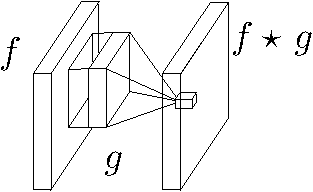
\includegraphics[scale=0.75]{fig/rel/imrecon/img/conv_schema.pdf}
    \end{columns}\pause
    \begin{center}
        {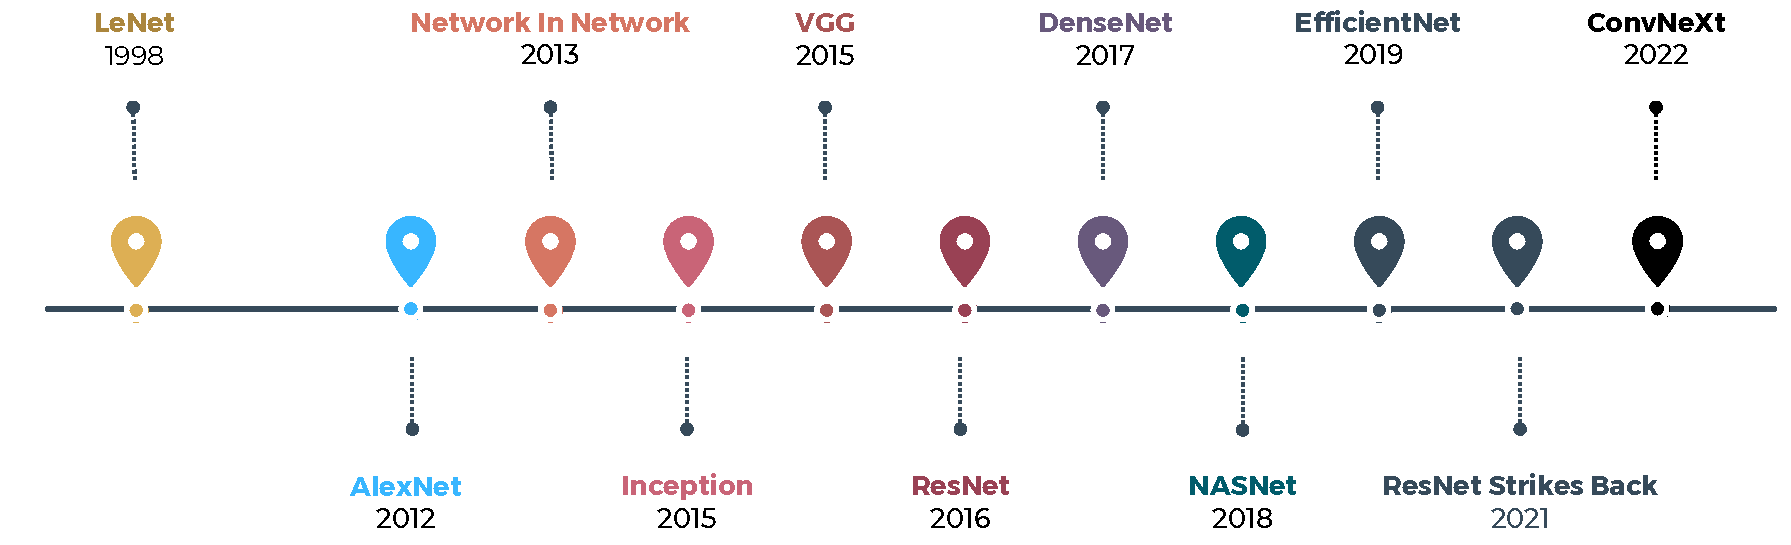
\includegraphics[width=\textwidth]{fig/rel/imrecon/img/CNN_timeline.pdf}}
    \end{center}
        
\end{frame}
%--------------------------------------------------------------------------------------------------
\begin{frame}[t]
    \frametitle{Image Recognition Models}
    \framesubtitle{Self Attention Architectures}
    \begin{columns}
        \column[T]{.5\textwidth}
         {\footnotesize Updates a representation, using the relevance of each element relative to others in an 
         embedding.\\
         An input is projected to three spaces ($Q K V$), the weights control the relevance of each 
         element.}
        \column[T]{.5\textwidth}
        \begin{center}
            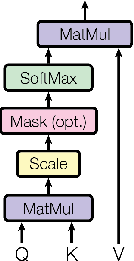
\includegraphics[width=0.5\textwidth]{fig/rel/imrecon/img/scaled_dotproduct.pdf}
        \end{center}
        
    \end{columns}
    
\end{frame}
%--------------------------------------------------------------------------------------------------
\begin{frame}[t]
    \frametitle{Image Recognition Models}
    \framesubtitle{The Current Landscape}
    Transformers had a strong impact on image recognition. 
    %--------------------------------------------------------------------------------------------------
\pgfplotstableread[col sep=comma,]{fig/rel/data/models_year.csv}\datatable
    \begin{tikzpicture}
        \begin{axis}[
            %font={\scriptsize},
            date coordinates in=x,
            date ZERO=2017-03-31,
            xtick distance=0.25,
            %xtick={\datatable}{Year},
            %xticklabel={\year-\month-\day},
            xtick=data,
            width=\textwidth,
            height=6.5cm,
            xticklabel style={rotate=90, anchor=near xticklabel},
            ylabel={Proportion of Papers (Quarterly)},
            legend style={at={(0, 1)}, anchor=north west},
            yticklabel style={/pgf/number format/fixed}
            ]
            \tikzstyle{every node}=[font=\scriptsize]
            \addplot [mark=*, red!80] table [x={Year}, y={ResNet}]{\datatable};
            \addlegendentry{{\tiny \Th{ResNet}}}

            \addplot [mark=*, black!80] table [x={Year}, y={VGG}]{\datatable};
            \addlegendentry{{\tiny \Th{VGG}}}

            \addplot [mark=*, green!80] table [x={Year}, y={DenseNet}]{\datatable};
            \addlegendentry{{\tiny\Th{DenseNet}}}

            \addplot [mark=*, cyan!80] table [x={Year}, y={EfficientNet}]{\datatable};
            \addlegendentry{{\tiny \Th{EfficientNet}}}

            \addplot [mark=*, blue!80] table [x={Year}, y={ViT}]{\datatable};
            \addlegendentry{{\tiny \Th{ViT}}}
        \end{axis}
    \end{tikzpicture}
%    \caption{\textbf{Proportion of articles published on ImageNet,} using image recognition models as backbone across the years. 
%             Original from \url{https://paperswithcode.com/method/resnet}}
%    \label{fig:paradigmn_shift}
%\end{figure}
    
\end{frame}